
\begin{table}
\caption{Overview of assimilation experiments performed.}
\centering
\begin{tabular}{llc}
Experiment name &  Assimilated Quantities  & Integration Time (Days) \\
\hline
NODA  &  none	& 81 				\\
AAM  &  $\chi_1$, $\chi_2$, $\Delta$LOD		& 81\\
RST  &  Radiosonde temperatures	& 31	\\
RST+AAM	 &  Radiosonde temperatures, $\chi_1$, $\chi_2$, $\Delta$LOD	& 17\\
\textcolor{unsure}{GPS-RO}	& \textcolor{unsure}{CHAMP-like GPS-RO refractivities} & \textcolor{alert}{FILL IN}	\\
\hline
\end{tabular}
%\tablenotetext{a}{Footnote text here.}
\label{tab:expts}
\end{table}

 \begin{figure}
\includegraphics[width=\textwidth]{../../Plots/ERP_DA/radiosonde_locations.pdf} 
 \caption{  }
 \label{fig:RS}
\end{figure}

 \begin{figure}
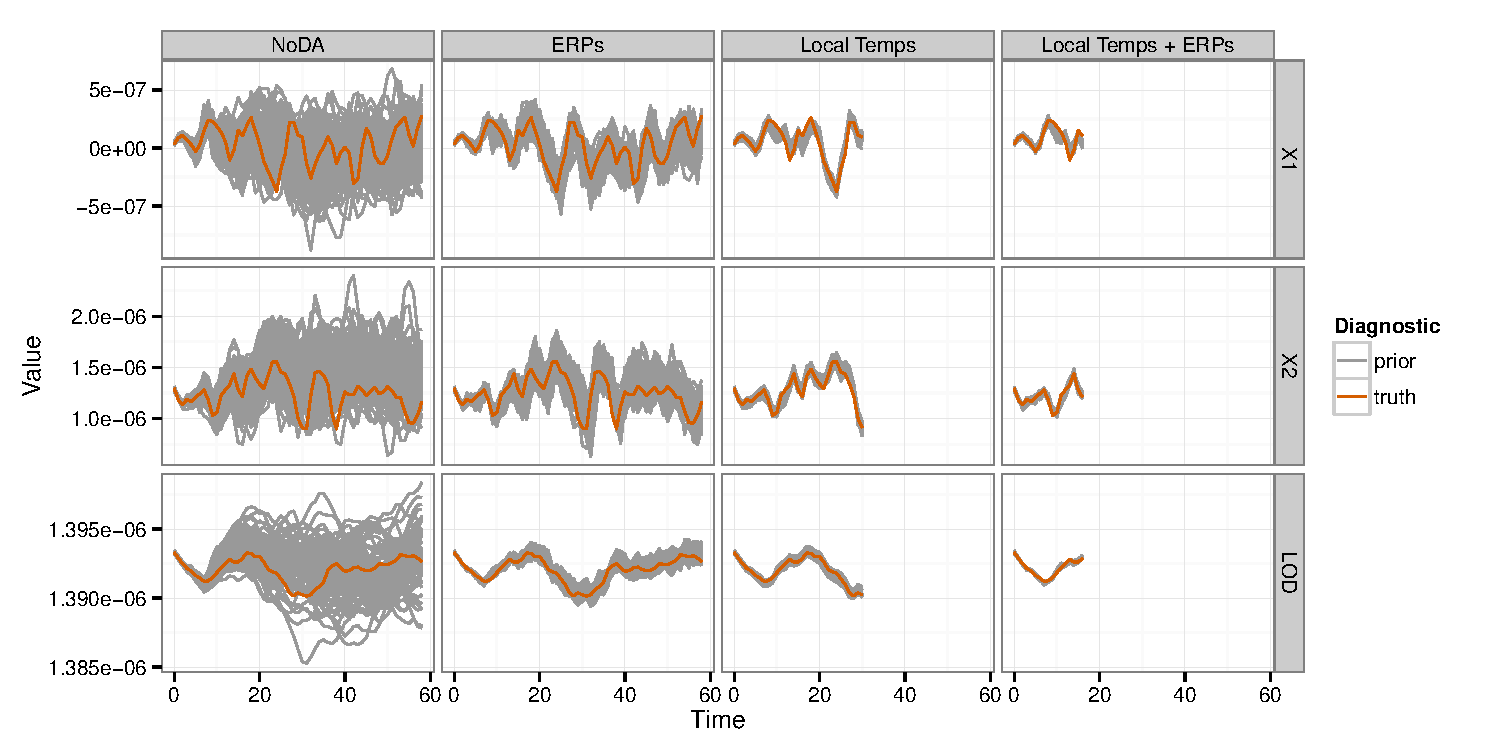
\includegraphics[width=\textwidth]{../../Plots/ERP_DA/paper/fit_to_ERPs.pdf} 
 \caption{ The DART prior ensemble (gray) compared to the true state (orange) in terms of assimilation time and each of the three angular momentum functions [(\ref{eq:X1})-(\ref{eq:X3}), (\ref{eq:X3_to_LOD})].  The columns compare the four experiments summarized in Table \ref{tab:expts}.  }
 \label{fig:fit_to_ERPs}
\end{figure}

 \begin{figure}
\includegraphics[width=\textwidth]{../../Plots/ERP_DA/paper/NODA_error_growth.pdf} 
 \caption{Top row: The mean square error in the ensemble mean zonal wind field as a function of vertical level and time (left), compared to the corresponding scaled ensemble spread (as in (\ref{eq:EvsS}), center), for the NoDA experiment.  Bottom row: as in the first row, but for surface pressure, and plotting over latitude and time. \textcolor{alert}{Changes: add letter labels.} }
 \label{fig:NODA}
\end{figure}
%BINK



 \begin{figure}
\includegraphics[width=\textwidth]{../../Plots/ERP_DA/paper/ERPALL_error_growth.pdf} 
 \caption{ Top row: The mean square error in the ensemble mean surface pressure field, and a function of latitude and time (left), compared to the corresponding scaled ensemble spread (as in (\ref{eq:EvsS}), center), for experiment AAM.  Bottom row: The difference between the surface pressure mean square error and ensemble spread fields in the AAM experiment, relative to the NoDA experiment.  \textcolor{alert}{To do: add letter labels here to make it easier to compare panels. }  }
 \label{fig:ERPDA_error_growth}
\end{figure}



\begin{figure}
\includegraphics[width=\textwidth]{../../Plots/ERP_DA/paper/rank_histogram_basic.pdf} 
 \caption{\textcolor{alert}{Rank histograms for surface pressure, counting over assimilation days 10-20 for (a) the NODA experiment, and (b) the AAM experiment.}}
 \label{fig:compare_divergence_basic}
\end{figure}

 \begin{figure}
\includegraphics[width=\textwidth]{../../Plots/ERP_DA/paper/RST_error_growth.pdf} 
 \caption{As in Figs. \ref{fig:NODA} and \ref{fig:ERPDA_error_growth}, but for experiment RST (assimilating radiosonde temperatures only).}
 \label{fig:RST}
\end{figure}

 \begin{figure}
\includegraphics[width=\textwidth]{../../Plots/ERP_DA/paper/REDUCTION2_error_growth.pdf} 
 \caption{As in Fig. \ref{fig:ERPDA_diff}, but now showing the differences between experiments AAM+RST and RST (positive values mean larger error or spread in experiment AAM+RST relative to RST).}
 \label{fig:ERPRST_diff}
\end{figure}

\begin{figure}
\includegraphics[width=\textwidth]{../../Plots/ERP_DA/paper/rank_histogram_added_value.pdf} 
 \caption{\textcolor{alert}{Replace this with rank histograms.}}
 \label{fig:compare_divergence_added_value}
\end{figure}

